% Options for packages loaded elsewhere
\PassOptionsToPackage{unicode}{hyperref}
\PassOptionsToPackage{hyphens}{url}
\PassOptionsToPackage{dvipsnames,svgnames,x11names}{xcolor}
%
\documentclass[
  letterpaper,
  DIV=11]{scrartcl}

\usepackage{amsmath,amssymb}
\usepackage{iftex}
\ifPDFTeX
  \usepackage[T1]{fontenc}
  \usepackage[utf8]{inputenc}
  \usepackage{textcomp} % provide euro and other symbols
\else % if luatex or xetex
  \usepackage{unicode-math}
  \defaultfontfeatures{Scale=MatchLowercase}
  \defaultfontfeatures[\rmfamily]{Ligatures=TeX,Scale=1}
\fi
\usepackage{lmodern}
\ifPDFTeX\else  
    % xetex/luatex font selection
\fi
% Use upquote if available, for straight quotes in verbatim environments
\IfFileExists{upquote.sty}{\usepackage{upquote}}{}
\IfFileExists{microtype.sty}{% use microtype if available
  \usepackage[]{microtype}
  \UseMicrotypeSet[protrusion]{basicmath} % disable protrusion for tt fonts
}{}
\makeatletter
\@ifundefined{KOMAClassName}{% if non-KOMA class
  \IfFileExists{parskip.sty}{%
    \usepackage{parskip}
  }{% else
    \setlength{\parindent}{0pt}
    \setlength{\parskip}{6pt plus 2pt minus 1pt}}
}{% if KOMA class
  \KOMAoptions{parskip=half}}
\makeatother
\usepackage{xcolor}
\setlength{\emergencystretch}{3em} % prevent overfull lines
\setcounter{secnumdepth}{-\maxdimen} % remove section numbering
% Make \paragraph and \subparagraph free-standing
\makeatletter
\ifx\paragraph\undefined\else
  \let\oldparagraph\paragraph
  \renewcommand{\paragraph}{
    \@ifstar
      \xxxParagraphStar
      \xxxParagraphNoStar
  }
  \newcommand{\xxxParagraphStar}[1]{\oldparagraph*{#1}\mbox{}}
  \newcommand{\xxxParagraphNoStar}[1]{\oldparagraph{#1}\mbox{}}
\fi
\ifx\subparagraph\undefined\else
  \let\oldsubparagraph\subparagraph
  \renewcommand{\subparagraph}{
    \@ifstar
      \xxxSubParagraphStar
      \xxxSubParagraphNoStar
  }
  \newcommand{\xxxSubParagraphStar}[1]{\oldsubparagraph*{#1}\mbox{}}
  \newcommand{\xxxSubParagraphNoStar}[1]{\oldsubparagraph{#1}\mbox{}}
\fi
\makeatother

\usepackage{color}
\usepackage{fancyvrb}
\newcommand{\VerbBar}{|}
\newcommand{\VERB}{\Verb[commandchars=\\\{\}]}
\DefineVerbatimEnvironment{Highlighting}{Verbatim}{commandchars=\\\{\}}
% Add ',fontsize=\small' for more characters per line
\usepackage{framed}
\definecolor{shadecolor}{RGB}{241,243,245}
\newenvironment{Shaded}{\begin{snugshade}}{\end{snugshade}}
\newcommand{\AlertTok}[1]{\textcolor[rgb]{0.68,0.00,0.00}{#1}}
\newcommand{\AnnotationTok}[1]{\textcolor[rgb]{0.37,0.37,0.37}{#1}}
\newcommand{\AttributeTok}[1]{\textcolor[rgb]{0.40,0.45,0.13}{#1}}
\newcommand{\BaseNTok}[1]{\textcolor[rgb]{0.68,0.00,0.00}{#1}}
\newcommand{\BuiltInTok}[1]{\textcolor[rgb]{0.00,0.23,0.31}{#1}}
\newcommand{\CharTok}[1]{\textcolor[rgb]{0.13,0.47,0.30}{#1}}
\newcommand{\CommentTok}[1]{\textcolor[rgb]{0.37,0.37,0.37}{#1}}
\newcommand{\CommentVarTok}[1]{\textcolor[rgb]{0.37,0.37,0.37}{\textit{#1}}}
\newcommand{\ConstantTok}[1]{\textcolor[rgb]{0.56,0.35,0.01}{#1}}
\newcommand{\ControlFlowTok}[1]{\textcolor[rgb]{0.00,0.23,0.31}{\textbf{#1}}}
\newcommand{\DataTypeTok}[1]{\textcolor[rgb]{0.68,0.00,0.00}{#1}}
\newcommand{\DecValTok}[1]{\textcolor[rgb]{0.68,0.00,0.00}{#1}}
\newcommand{\DocumentationTok}[1]{\textcolor[rgb]{0.37,0.37,0.37}{\textit{#1}}}
\newcommand{\ErrorTok}[1]{\textcolor[rgb]{0.68,0.00,0.00}{#1}}
\newcommand{\ExtensionTok}[1]{\textcolor[rgb]{0.00,0.23,0.31}{#1}}
\newcommand{\FloatTok}[1]{\textcolor[rgb]{0.68,0.00,0.00}{#1}}
\newcommand{\FunctionTok}[1]{\textcolor[rgb]{0.28,0.35,0.67}{#1}}
\newcommand{\ImportTok}[1]{\textcolor[rgb]{0.00,0.46,0.62}{#1}}
\newcommand{\InformationTok}[1]{\textcolor[rgb]{0.37,0.37,0.37}{#1}}
\newcommand{\KeywordTok}[1]{\textcolor[rgb]{0.00,0.23,0.31}{\textbf{#1}}}
\newcommand{\NormalTok}[1]{\textcolor[rgb]{0.00,0.23,0.31}{#1}}
\newcommand{\OperatorTok}[1]{\textcolor[rgb]{0.37,0.37,0.37}{#1}}
\newcommand{\OtherTok}[1]{\textcolor[rgb]{0.00,0.23,0.31}{#1}}
\newcommand{\PreprocessorTok}[1]{\textcolor[rgb]{0.68,0.00,0.00}{#1}}
\newcommand{\RegionMarkerTok}[1]{\textcolor[rgb]{0.00,0.23,0.31}{#1}}
\newcommand{\SpecialCharTok}[1]{\textcolor[rgb]{0.37,0.37,0.37}{#1}}
\newcommand{\SpecialStringTok}[1]{\textcolor[rgb]{0.13,0.47,0.30}{#1}}
\newcommand{\StringTok}[1]{\textcolor[rgb]{0.13,0.47,0.30}{#1}}
\newcommand{\VariableTok}[1]{\textcolor[rgb]{0.07,0.07,0.07}{#1}}
\newcommand{\VerbatimStringTok}[1]{\textcolor[rgb]{0.13,0.47,0.30}{#1}}
\newcommand{\WarningTok}[1]{\textcolor[rgb]{0.37,0.37,0.37}{\textit{#1}}}

\providecommand{\tightlist}{%
  \setlength{\itemsep}{0pt}\setlength{\parskip}{0pt}}\usepackage{longtable,booktabs,array}
\usepackage{calc} % for calculating minipage widths
% Correct order of tables after \paragraph or \subparagraph
\usepackage{etoolbox}
\makeatletter
\patchcmd\longtable{\par}{\if@noskipsec\mbox{}\fi\par}{}{}
\makeatother
% Allow footnotes in longtable head/foot
\IfFileExists{footnotehyper.sty}{\usepackage{footnotehyper}}{\usepackage{footnote}}
\makesavenoteenv{longtable}
\usepackage{graphicx}
\makeatletter
\newsavebox\pandoc@box
\newcommand*\pandocbounded[1]{% scales image to fit in text height/width
  \sbox\pandoc@box{#1}%
  \Gscale@div\@tempa{\textheight}{\dimexpr\ht\pandoc@box+\dp\pandoc@box\relax}%
  \Gscale@div\@tempb{\linewidth}{\wd\pandoc@box}%
  \ifdim\@tempb\p@<\@tempa\p@\let\@tempa\@tempb\fi% select the smaller of both
  \ifdim\@tempa\p@<\p@\scalebox{\@tempa}{\usebox\pandoc@box}%
  \else\usebox{\pandoc@box}%
  \fi%
}
% Set default figure placement to htbp
\def\fps@figure{htbp}
\makeatother

\KOMAoption{captions}{tableheading}
\makeatletter
\@ifpackageloaded{caption}{}{\usepackage{caption}}
\AtBeginDocument{%
\ifdefined\contentsname
  \renewcommand*\contentsname{Inhaltsverzeichnis}
\else
  \newcommand\contentsname{Inhaltsverzeichnis}
\fi
\ifdefined\listfigurename
  \renewcommand*\listfigurename{Abbildungsverzeichnis}
\else
  \newcommand\listfigurename{Abbildungsverzeichnis}
\fi
\ifdefined\listtablename
  \renewcommand*\listtablename{Tabellenverzeichnis}
\else
  \newcommand\listtablename{Tabellenverzeichnis}
\fi
\ifdefined\figurename
  \renewcommand*\figurename{Abbildung}
\else
  \newcommand\figurename{Abbildung}
\fi
\ifdefined\tablename
  \renewcommand*\tablename{Tabelle}
\else
  \newcommand\tablename{Tabelle}
\fi
}
\@ifpackageloaded{float}{}{\usepackage{float}}
\floatstyle{ruled}
\@ifundefined{c@chapter}{\newfloat{codelisting}{h}{lop}}{\newfloat{codelisting}{h}{lop}[chapter]}
\floatname{codelisting}{Listing}
\newcommand*\listoflistings{\listof{codelisting}{Listingverzeichnis}}
\makeatother
\makeatletter
\makeatother
\makeatletter
\@ifpackageloaded{caption}{}{\usepackage{caption}}
\@ifpackageloaded{subcaption}{}{\usepackage{subcaption}}
\makeatother

\ifLuaTeX
\usepackage[bidi=basic]{babel}
\else
\usepackage[bidi=default]{babel}
\fi
\babelprovide[main,import]{ngerman}
% get rid of language-specific shorthands (see #6817):
\let\LanguageShortHands\languageshorthands
\def\languageshorthands#1{}
\ifLuaTeX
  \usepackage[german]{selnolig} % disable illegal ligatures
\fi
\usepackage{bookmark}

\IfFileExists{xurl.sty}{\usepackage{xurl}}{} % add URL line breaks if available
\urlstyle{same} % disable monospaced font for URLs
\hypersetup{
  pdftitle={Datenanalyse umwelt.info:   Von Rohdaten zu Projekten},
  pdfauthor={Tim Fangmeyer linkedin/today/author/timfangmeyer},
  pdflang={de},
  colorlinks=true,
  linkcolor={blue},
  filecolor={Maroon},
  citecolor={Blue},
  urlcolor={Blue},
  pdfcreator={LaTeX via pandoc}}


\title{Datenanalyse umwelt.info: Von Rohdaten zu Projekten}
\author{Tim Fangmeyer\\
\textbf{linkedin/today/author/timfangmeyer}}
\date{}

\begin{document}
\maketitle


\subsection{umwelt.info}\label{umwelt.info}

Stellt die Daten sowohl über die Suche \ldots{}

\pandocbounded{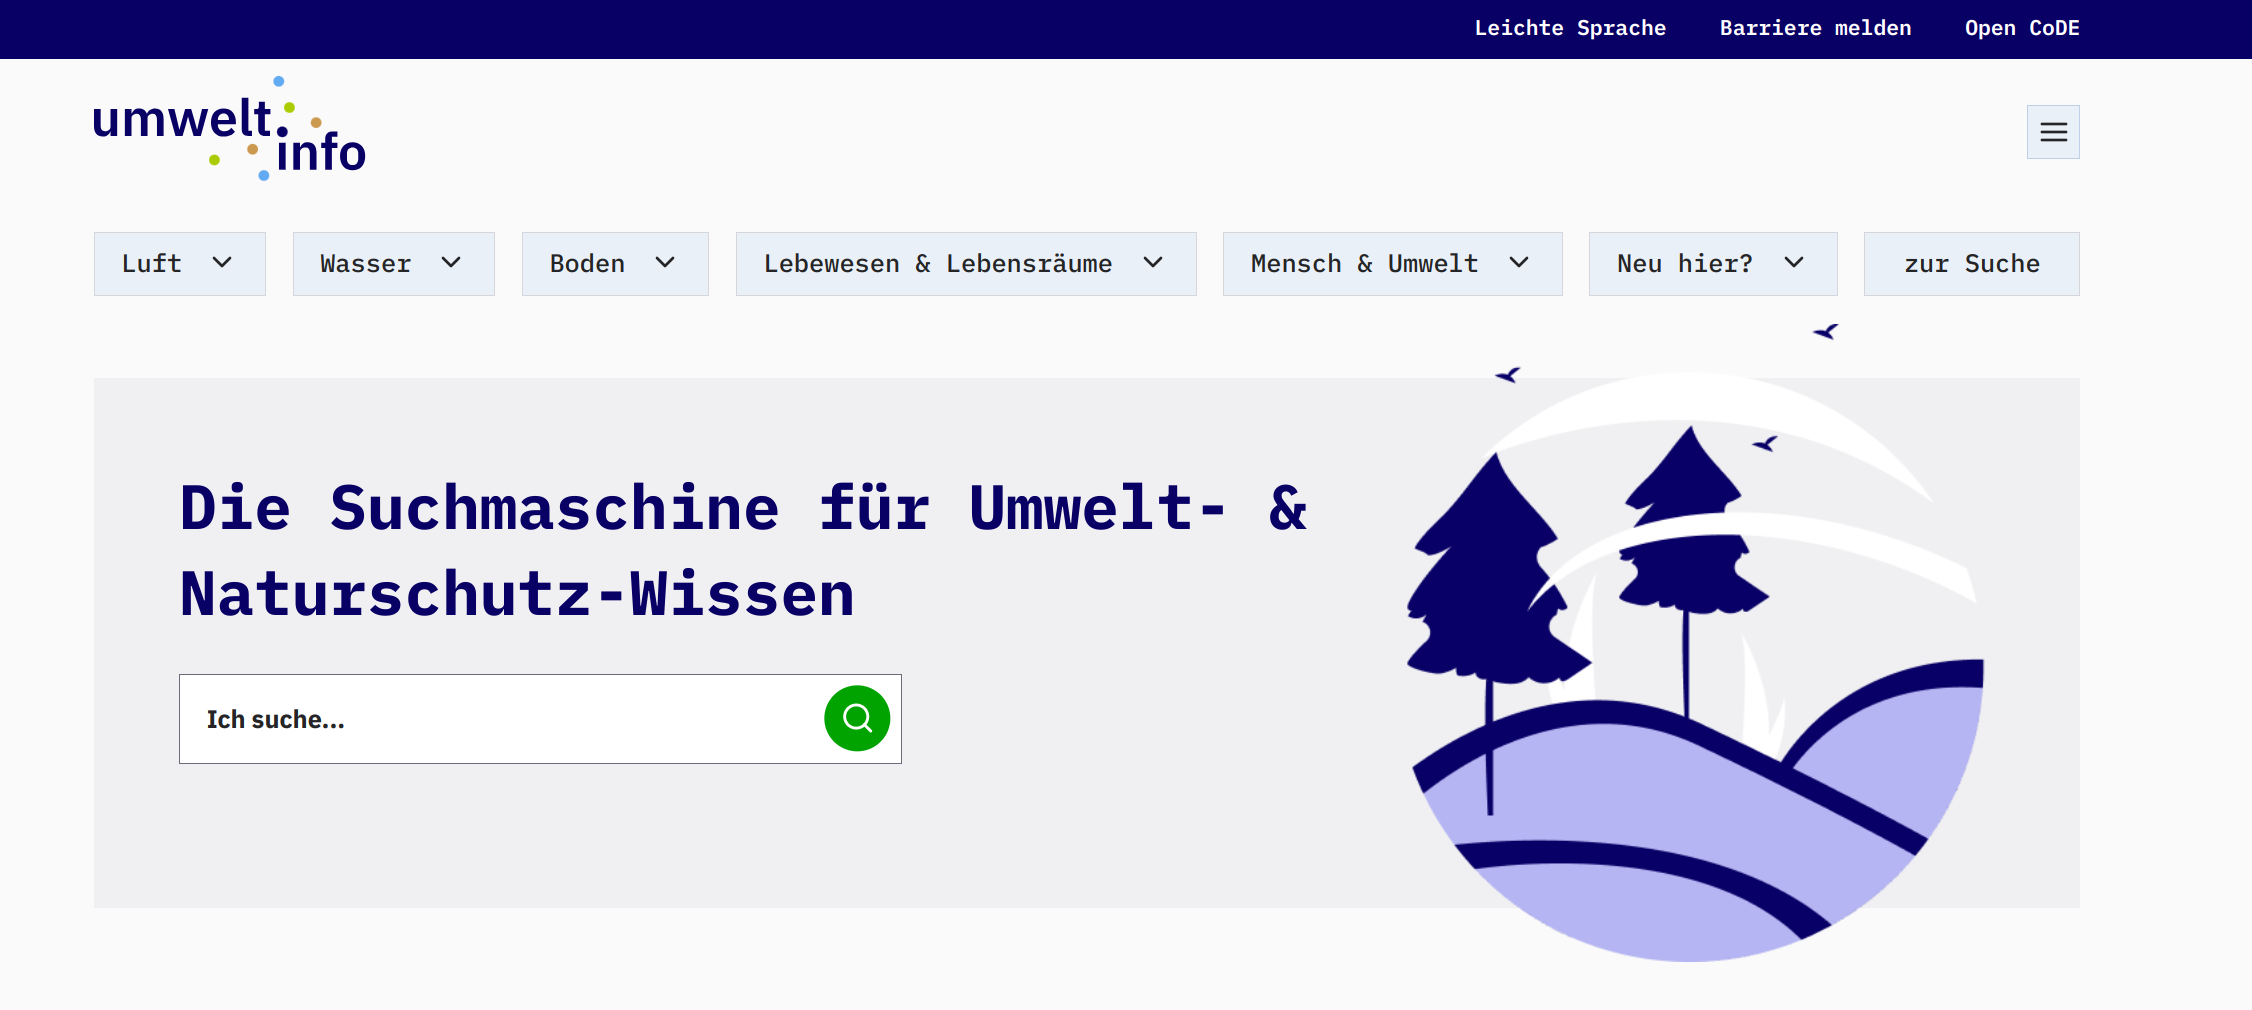
\includegraphics[keepaspectratio]{images/suche.png}}

\subsection{}\label{section}

\ldots{} als auch über eine Schnittstelle bereit.
\pandocbounded{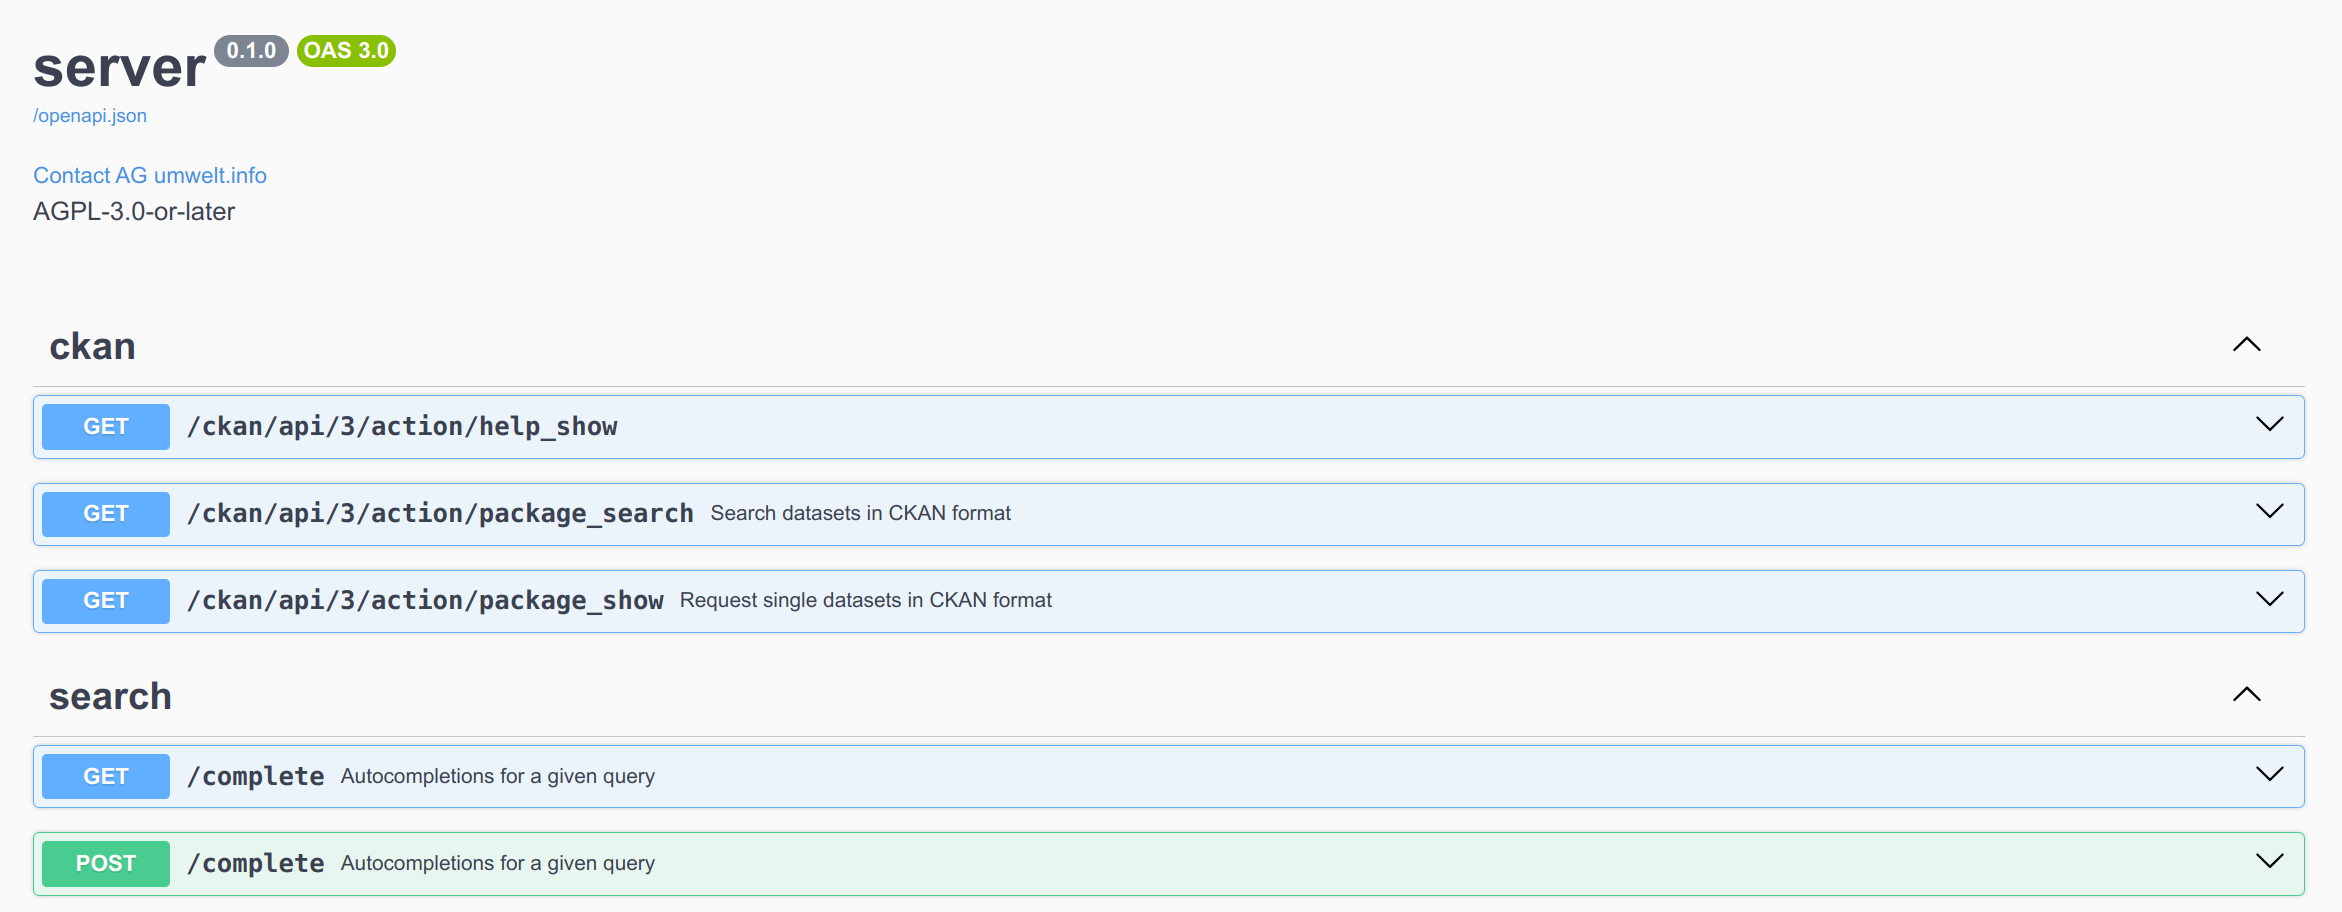
\includegraphics[keepaspectratio]{images/schnistellen_uebersicht.png}}

\subsection{Web-UI vs.~API-Zugriff}\label{web-ui-vs.-api-zugriff}

\subsubsection{🌐 Web-Oberfläche
(umwelt.info)}\label{web-oberfluxe4che-umwelt.info}

\begin{itemize}
\tightlist
\item
  Intuitives Erkunden und Filtern der Daten
\item
  ABER: ``Händische'' Arbeit nötig, nicht automatisierbar
\end{itemize}

\subsubsection{🔌 API-Zugriff}\label{api-zugriff}

\begin{itemize}
\tightlist
\item
  Automatisierung möglich (Scripting, regelmäßige Updates)
\item
  Verarbeitung großer Datenmengen
\item
  ABER: Technisches Know-how erforderlich
\end{itemize}

\subsection{Wir sind hier:
Metadaten-Exploration}\label{wir-sind-hier-metadaten-exploration}

\begin{enumerate}
\def\labelenumi{\arabic{enumi}.}
\tightlist
\item
  ✅ \textbf{Katalog durchsuchen}
\item
  ✅ \textbf{Metadaten abrufen}
\item
  ⬜ \textbf{Eigentliche Daten herunterladen}
\item
  ⬜ \textbf{Daten reinigen, aggregieren, analysieren, visualisieren,
  etc.}
\end{enumerate}

\begin{quote}
💡 \textbf{Wichtig:} Die folgenden API-Beispiele zeigen nur die
\emph{Suche und Beschreibung} der Daten.
\end{quote}

\subsection{API}\label{api}

Programmierschnittstellen (APIs) ermöglichen Dritten den Zugang zu
vorher verschlossenen Datenpools.
\pandocbounded{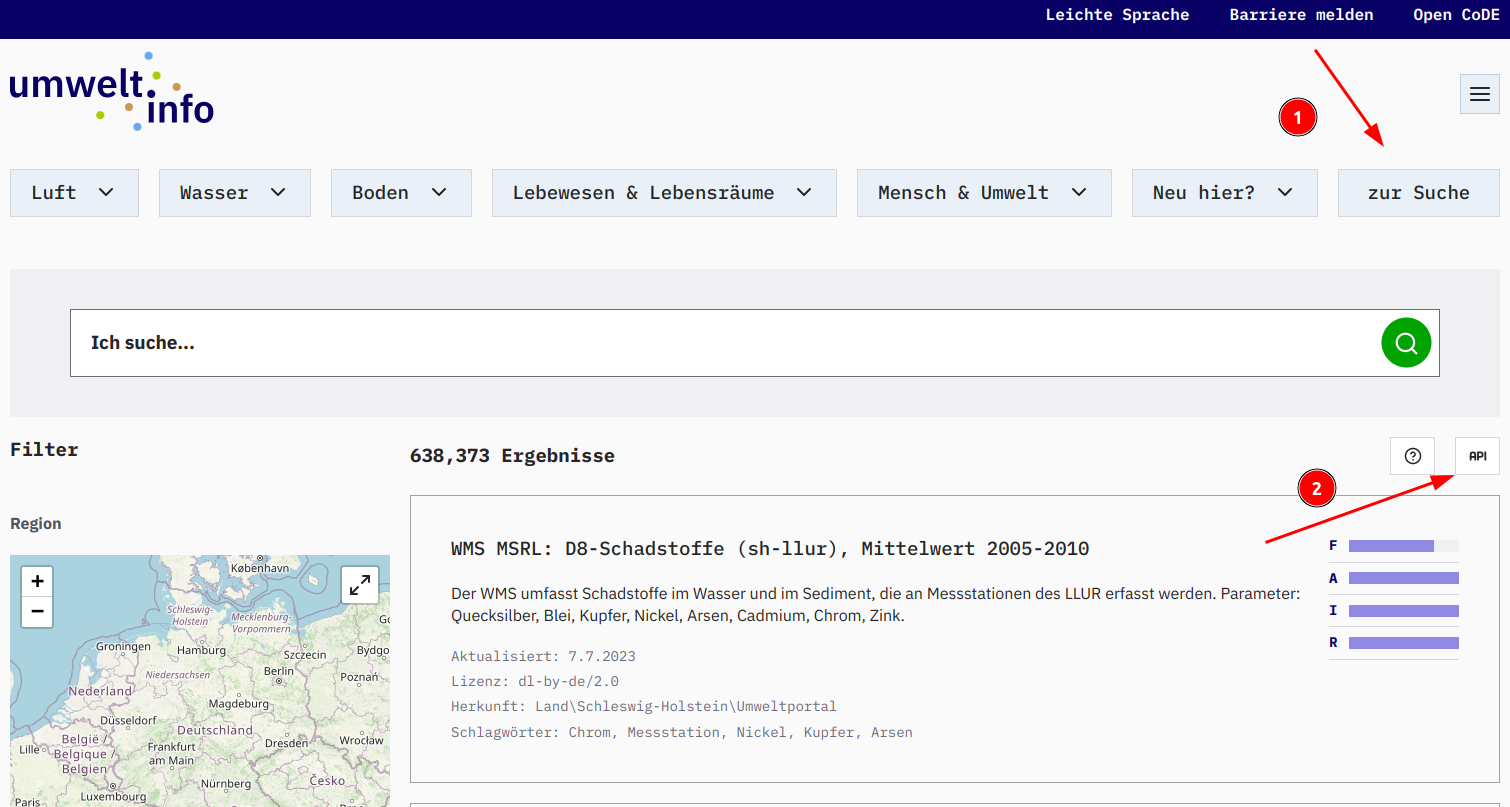
\includegraphics[keepaspectratio]{images/api.png}}

\subsection{Swagger-UI}\label{swagger-ui}

Interaktive Dokumentation für REST-APIs. Mit Swagger UI können
Entwickler die verfügbaren API-Endpunkte direkt im Browser erkunden.
\pandocbounded{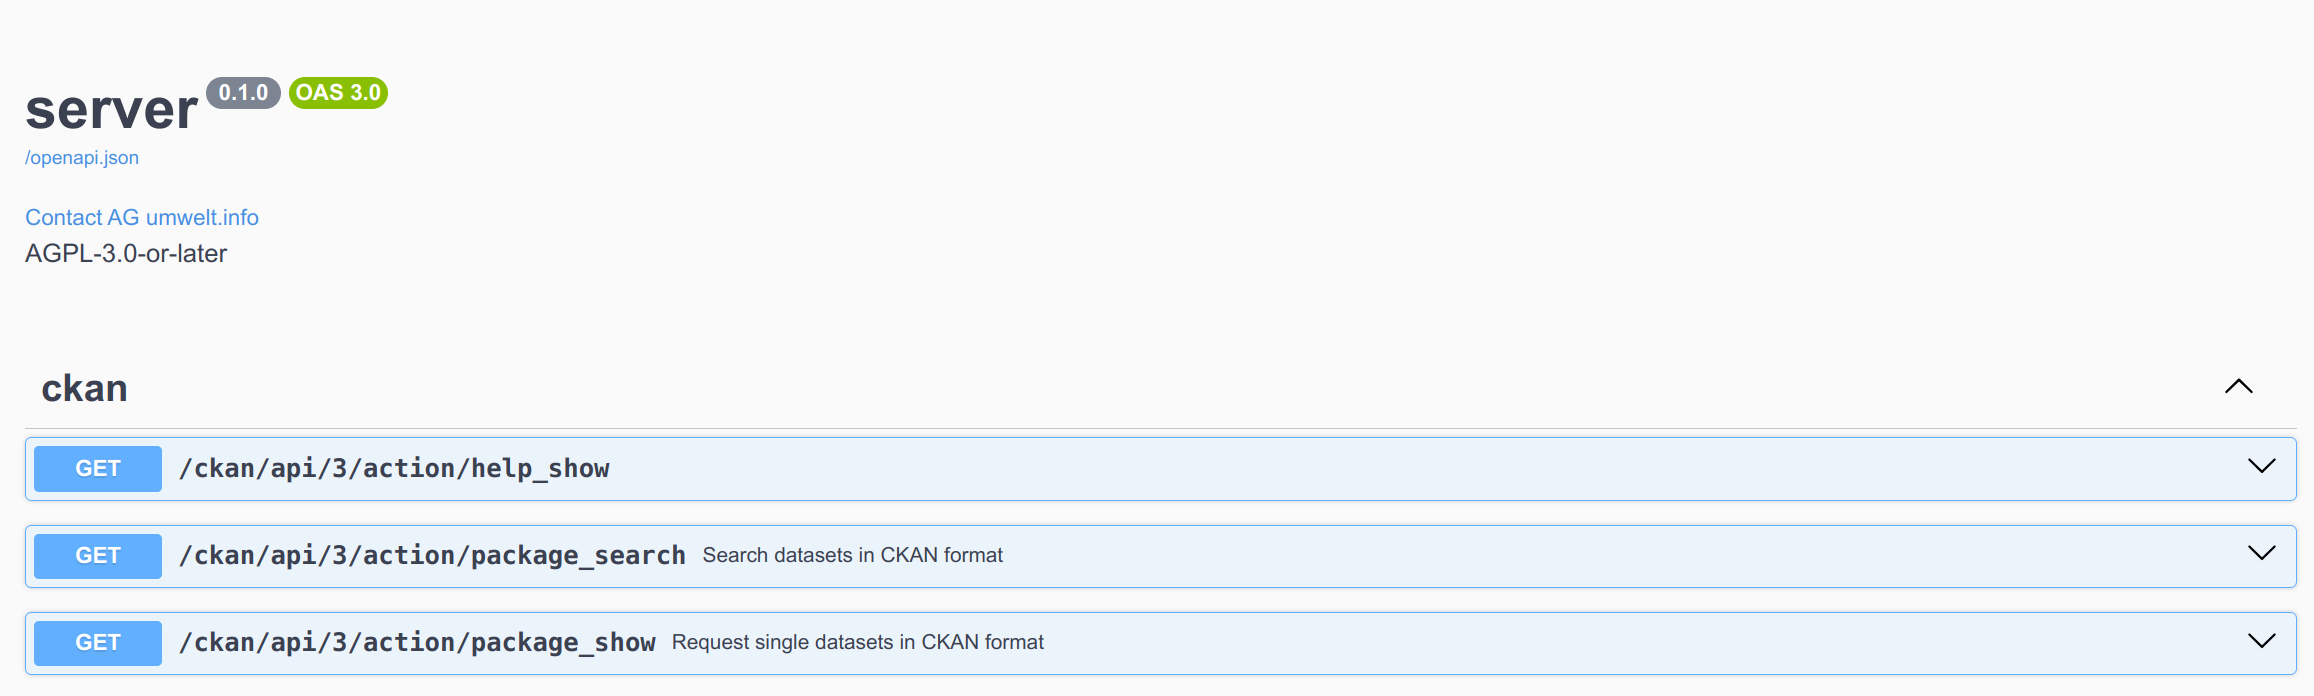
\includegraphics[keepaspectratio]{images/swagger_ui.png}}
\href{https://md.umwelt.info/swagger-ui/}{swagger-ui/}

\subsection{Umfang der Schnittstelle}\label{umfang-der-schnittstelle}

Wichtigste Endpunkte:

\begin{itemize}
\tightlist
\item
  \textbf{Volltextsuche} über alle Datensätze (+ Filteroptionen)
\item
  \textbf{Einzeldatensatz-Abruf} detaillierter Metadaten
\item
  \textbf{Statistik-Endpunkt} für Nutzungsstatistiken
\end{itemize}

\subsection{API: Wichtige CKAN-Endpunkte für die Abfrage von
umwelt.info}\label{api-wichtige-ckan-endpunkte-fuxfcr-die-abfrage-von-umwelt.info}

\begin{itemize}
\tightlist
\item
  \textbf{\texttt{/package\_search}} Volltextsuche nach Suchbegriff. Die
  Wildcard ``*'' ermöglicht die Abfrage des gesamten Metadatenbestandes
\item
  \textbf{\texttt{/package\_show}} Ermöglicht die Abfrage einzelner
  Datensätze im CKAN Format. - \textbf{\texttt{/counts/now}}: Aktuelle
  Gesamtzahl an Datensätzen.
\item
  \textbf{\texttt{/counts/now}}: Aktuelle Gesamtzahl an Datensätzen.
\end{itemize}

\subsection{API Beispiele mit Python}\label{api-beispiele-mit-python}

Beispielshafte Abfrage der CKAN-API mit Python. \begin{center}

\includegraphics[width=0.35\linewidth,height=0.35\textheight]{images/python_logo.png}
\end{center}

\subsection{\texorpdfstring{API Endpoint: \textbf{\texttt{/counts/now}}
📈}{API Endpoint: /counts/now 📈}}\label{api-endpoint-countsnow}

\begin{Shaded}
\begin{Highlighting}[]
\ImportTok{import}\NormalTok{ requests}

\NormalTok{url }\OperatorTok{=} \StringTok{"https://md.umwelt.info/counts/now"}
\NormalTok{response }\OperatorTok{=}\NormalTok{ requests.get(url)}
\NormalTok{data }\OperatorTok{=}\NormalTok{ response.json()}

\CommentTok{\# Ausgabe der Antwort}
\BuiltInTok{print}\NormalTok{(data)}
\end{Highlighting}
\end{Shaded}

\begin{Shaded}
\begin{Highlighting}[]
\CommentTok{\# Beispiel{-}Output:}
\NormalTok{\{}
    \StringTok{"datasets"}\NormalTok{: }\DecValTok{638373}\NormalTok{,}
    \StringTok{"sources"}\NormalTok{: }\DecValTok{129}\NormalTok{,}
    \StringTok{"providers"}\NormalTok{: }\DecValTok{45}\NormalTok{,}
    \StringTok{"failed\_harvests"}\NormalTok{: }\DecValTok{0}\NormalTok{,}
    \StringTok{"errors"}\NormalTok{: }\DecValTok{900}
\NormalTok{\}}
\end{Highlighting}
\end{Shaded}

\subsection{\texorpdfstring{API Endpoint:
\textbf{\texttt{/package\_search}}
🔍}{API Endpoint: /package\_search 🔍}}\label{api-endpoint-package_search}

Request

\begin{Shaded}
\begin{Highlighting}[]
\ImportTok{import}\NormalTok{ requests}

\CommentTok{\# API{-}Parameter}
\NormalTok{base\_url }\OperatorTok{=} \StringTok{"https://md.umwelt.info/ckan/api/3/action/package\_search"}
\NormalTok{params }\OperatorTok{=}\NormalTok{ \{}
    \StringTok{"q"}\NormalTok{: }\StringTok{"Grundwasserpegel"}\NormalTok{,  }\CommentTok{\# Suchbegriff}
    \StringTok{"rows"}\NormalTok{: }\DecValTok{1}                 \CommentTok{\# Anzahl der Ergebnisse}
\NormalTok{\}}

\CommentTok{\# API{-}Abfrage durchführen}
\NormalTok{response }\OperatorTok{=}\NormalTok{ requests.get(base\_url, params}\OperatorTok{=}\NormalTok{params)}
\NormalTok{data }\OperatorTok{=}\NormalTok{ response.json()}
\end{Highlighting}
\end{Shaded}

\subsection{\texorpdfstring{API Endpoint:
\textbf{\texttt{/package\_search}}}{API Endpoint: /package\_search}}\label{api-endpoint-package_search-1}

Result

\begin{Shaded}
\begin{Highlighting}[]
\CommentTok{\# Beispiel{-}Output:}
\NormalTok{\{}
    \StringTok{"help"}\NormalTok{: }\StringTok{"/api/3/action/help\_show?name=package\_search"}\NormalTok{,}
    \StringTok{"success"}\NormalTok{: true,}
    \StringTok{"result"}\NormalTok{: \{}
        \StringTok{"count"}\NormalTok{: }\DecValTok{81765}\NormalTok{,}
        \StringTok{"facets"}\NormalTok{: [],}
        \StringTok{"search\_facets"}\NormalTok{: [],}
        \StringTok{"sort"}\NormalTok{: }\StringTok{"score desc"}\NormalTok{,}
        \StringTok{"results"}\NormalTok{: [}
\NormalTok{            \{}
                \StringTok{"id"}\NormalTok{: }\StringTok{"**Z292ZGF0YS8xZjM2ZGRhYS0xZGM4LTQ4YWYtOWEyMS1iNmVjZmFlZjExNzk=**"}\NormalTok{,}
                \StringTok{"name"}\NormalTok{: }\StringTok{"govdata/1f36ddaa{-}1dc8{-}48af{-}9a21{-}b6ecfaef1179"}\NormalTok{,}
                \StringTok{"title"}\NormalTok{: }\StringTok{"Grundwasserpegelmessung in Stadt und Landkreis in Osnabrück"}\NormalTok{,}
                \StringTok{"private"}\NormalTok{: false,}
                \StringTok{"license\_url"}\NormalTok{: }\StringTok{"https://www.govdata.de/dl{-}de/by{-}2{-}0"}\NormalTok{,}
                \StringTok{"license\_title"}\NormalTok{: }\StringTok{"dl{-}by{-}de/2.0"}
\NormalTok{                ...}
\NormalTok{            \}}
\NormalTok{        ]}
\NormalTok{    \}}
\NormalTok{\}}
\end{Highlighting}
\end{Shaded}

\subsection{\texorpdfstring{API Endpoint:
\textbf{\texttt{/package\_show}}
📦}{API Endpoint: /package\_show 📦}}\label{api-endpoint-package_show}

Request

\begin{Shaded}
\begin{Highlighting}[]
\ImportTok{import}\NormalTok{ requests}

\CommentTok{\# API{-}Parameter}
\NormalTok{base\_url }\OperatorTok{=} \StringTok{"https://md.umwelt.info/ckan/api/3/action/package\_show"}
\NormalTok{dataset\_id }\OperatorTok{=} \StringTok{"Z292ZGF0YS8xZjM2ZGRhYS0xZGM4LTQ4YWYtOWEyMS1iNmVjZmFlZjExNzk="}
\NormalTok{params }\OperatorTok{=}\NormalTok{ \{}\StringTok{"id"}\NormalTok{: dataset\_id\}}

\CommentTok{\# API{-}Abfrage durchführen}
\NormalTok{response }\OperatorTok{=}\NormalTok{ requests.get(base\_url, params}\OperatorTok{=}\NormalTok{params)}
\NormalTok{data }\OperatorTok{=}\NormalTok{ response.json()}
\end{Highlighting}
\end{Shaded}

\subsection{\texorpdfstring{API Endpoint:
\textbf{\texttt{/package\_show}}
📦}{API Endpoint: /package\_show 📦}}\label{api-endpoint-package_show-1}

Result

\begin{Shaded}
\begin{Highlighting}[]
\CommentTok{\# Beispiel{-}Output:}
\NormalTok{\{}
    \StringTok{"help"}\NormalTok{: }\StringTok{"/api/3/action/help\_show?name=package\_show"}\NormalTok{,}
    \StringTok{"success"}\NormalTok{: true,}
    \StringTok{"result"}\NormalTok{: \{}
        \StringTok{"id"}\NormalTok{: }\StringTok{"Z292ZGF0YS8xZjM2ZGRhYS0xZGM4LTQ4YWYtOWEyMS1iNmVjZmFlZjExNzk="}\NormalTok{,}
        \StringTok{"name"}\NormalTok{: }\StringTok{"govdata/1f36ddaa{-}1dc8{-}48af{-}9a21{-}b6ecfaef1179"}\NormalTok{,}
        \StringTok{"title"}\NormalTok{: }\StringTok{"Grundwasserpegelmessung in Stadt und Landkreis in Osnabrück"}\NormalTok{,}
        \StringTok{"private"}\NormalTok{: false,}
        \StringTok{"license\_url"}\NormalTok{: }\StringTok{"https://www.govdata.de/dl{-}de/by{-}2{-}0"}\NormalTok{,}
        \StringTok{"license\_title"}\NormalTok{: }\StringTok{"dl{-}by{-}de/2.0"}\NormalTok{,}
        \StringTok{"notes"}\NormalTok{: }\StringTok{"An mehreren Stellen in Stadt und Landkreis Osnabrück werden Grundwasserpegel automatisiert mithilfe von Sensoren erfasst."}
\NormalTok{    \}}
\NormalTok{\}}
\end{Highlighting}
\end{Shaded}

\subsection{Praxisprojekt:
Grundwasser-Atlas}\label{praxisprojekt-grundwasser-atlas}

Das Journalismuskokllektiv CORRECTIV mit einer interaktiven Karte einen
Überblick, wo in Deutschland das Grundwasser seit 1990 sinkt, gleich
bleibt oder steigt.

Quelle:
\href{https://correctiv.org/aktuelles/kampf-um-wasser/2022/10/25/klimawandel-grundwasser-in-deutschland-sinkt/}{CORRECTIV}

\subsection{Interaktive Karte mit
Lokalbezug}\label{interaktive-karte-mit-lokalbezug}

\pandocbounded{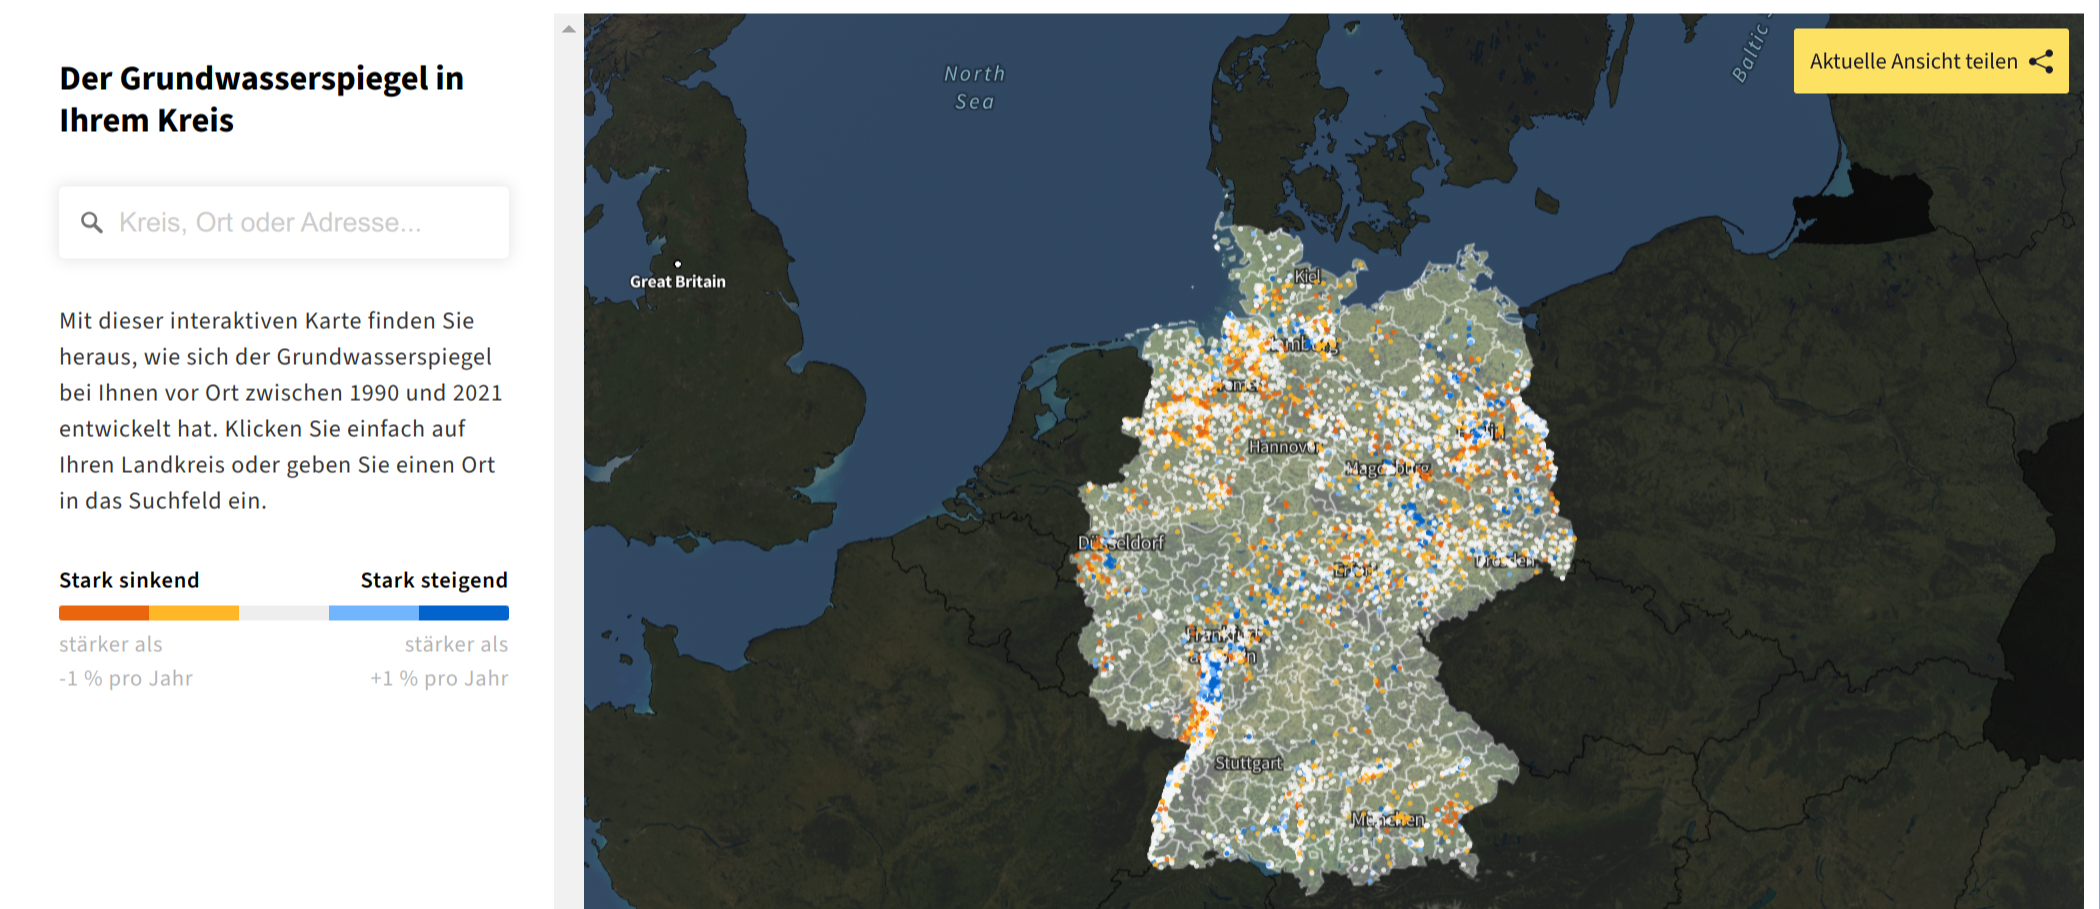
\includegraphics[keepaspectratio]{images/correctiv_karte.png}}

Quelle:
\href{https://correctiv.org/aktuelles/kampf-um-wasser/2022/10/25/klimawandel-grundwasser-in-deutschland-sinkt/}{CORRECTIV}

\subsection{Vorgehen beim
Grundwasser-Atlas}\label{vorgehen-beim-grundwasser-atlas}

\begin{itemize}
\tightlist
\item
  Abruf der der Positionen aller Grundwassermessstellen
\item
  Abruf der jeweiligen Pegelstände 1990-2021
\item
  Datenreinigung, Normalisierung, Trendberechnung, Visualisierung
\end{itemize}

\subsection{Welche Probleme können bei der Analyse
auftreten?}\label{welche-probleme-kuxf6nnen-bei-der-analyse-auftreten}

\begin{itemize}
\tightlist
\item
  Daten nicht vorhanden oder nicht unter Open-Data-Lizenz
\item
  Messwerte vorhanden, aber die Position der Messstellen nicht
  (Anonymisierung)
\item
  Messstellen werden in unterschiedlichen Zeiträumen gemessen
\end{itemize}

\subsection{Praxisbeispiel: Abruf Grundwassermessstellen
Berlin}\label{praxisbeispiel-abruf-grundwassermessstellen-berlin}

\begin{itemize}
\tightlist
\item
  Praktische Demonstration anhand eines Bundeslandes
\item
  Suche über das Portal nach den Berliner Grundwasser-Messstellen
\end{itemize}

\subsection{Praxisbeispiel: Abruf Grundwassermessstellen
Berlin}\label{praxisbeispiel-abruf-grundwassermessstellen-berlin-1}

\pandocbounded{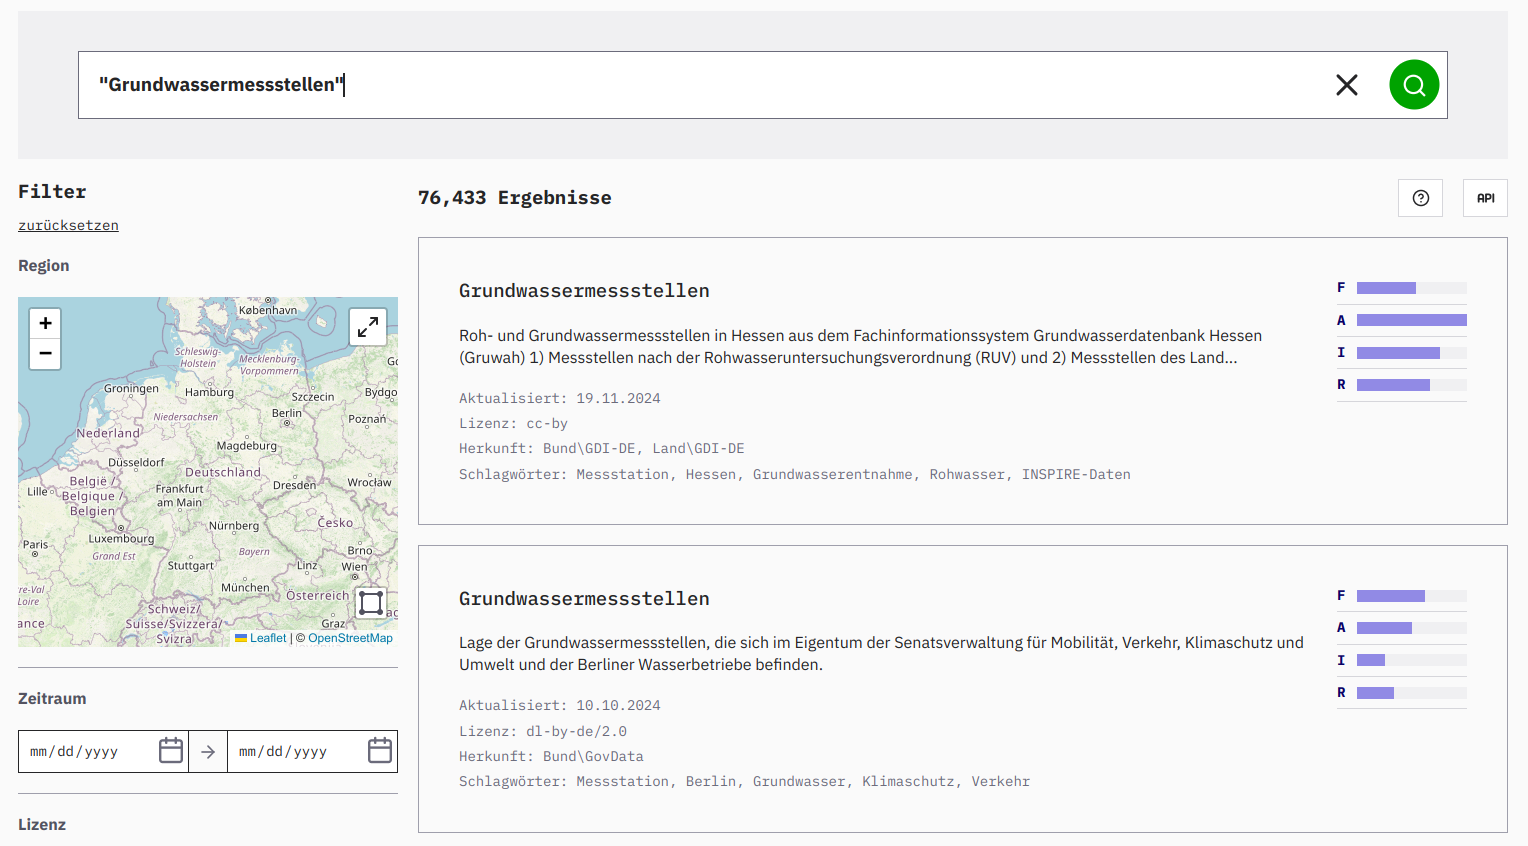
\includegraphics[keepaspectratio]{images/grundwassermessstellen_berlin.png}}

\subsection{Grundwassermessstellen als
WFS-Daten}\label{grundwassermessstellen-als-wfs-daten}

Web Feature Services sind Webschnittstellen, die den direkten Zugriff
auf raumbezogene Daten ermöglichen.

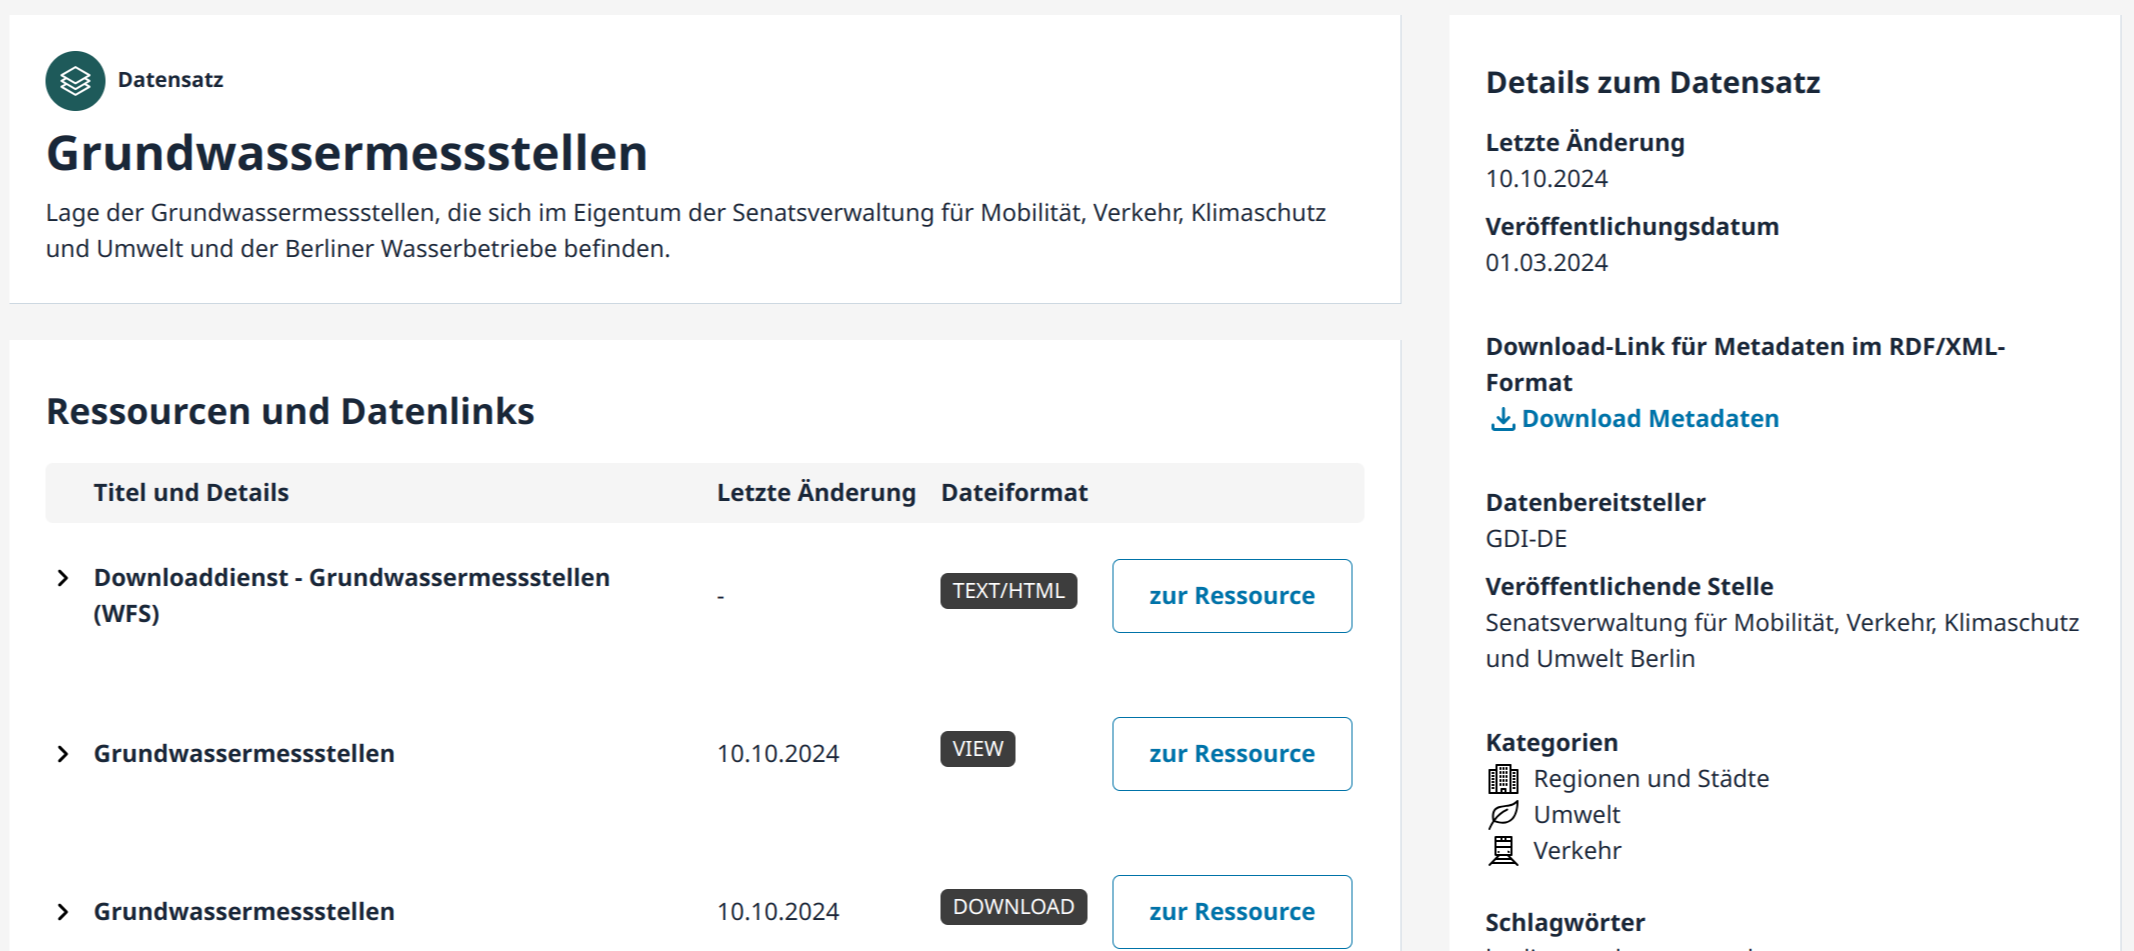
\includegraphics[width=0.7\linewidth,height=0.7\textheight]{images/govdata_grundwassermessstellen.png}

Quelle:
\href{https://www.govdata.de/suche/daten/grundwassermessstellen}{GovData}

\subsection{Abruf der WFS-Daten mit
Python}\label{abruf-der-wfs-daten-mit-python}

Request

\begin{Shaded}
\begin{Highlighting}[]
\ImportTok{import}\NormalTok{ requests}
\ImportTok{import}\NormalTok{ json}

\NormalTok{url }\OperatorTok{=} \StringTok{"https://gdi.berlin.de/services/wfs/gwm"}
\NormalTok{params }\OperatorTok{=}\NormalTok{ \{}
    \StringTok{\textquotesingle{}SERVICE\textquotesingle{}}\NormalTok{: }\StringTok{\textquotesingle{}WFS\textquotesingle{}}\NormalTok{,}
    \StringTok{\textquotesingle{}VERSION\textquotesingle{}}\NormalTok{: }\StringTok{\textquotesingle{}2.0.0\textquotesingle{}}\NormalTok{,}
    \StringTok{\textquotesingle{}REQUEST\textquotesingle{}}\NormalTok{: }\StringTok{\textquotesingle{}GetFeature\textquotesingle{}}\NormalTok{,}
    \StringTok{\textquotesingle{}TYPENAMES\textquotesingle{}}\NormalTok{: }\StringTok{\textquotesingle{}gwm:grundwassermessstellen\textquotesingle{}}\NormalTok{,}
    \StringTok{\textquotesingle{}OUTPUTFORMAT\textquotesingle{}}\NormalTok{: }\StringTok{\textquotesingle{}application/json\textquotesingle{}}
\NormalTok{\}}

\NormalTok{response }\OperatorTok{=}\NormalTok{ requests.get(url, params}\OperatorTok{=}\NormalTok{params)}
\NormalTok{data }\OperatorTok{=}\NormalTok{ response.json()}

\BuiltInTok{print}\NormalTok{(json.dumps(data, indent}\OperatorTok{=}\DecValTok{2}\NormalTok{))}
\end{Highlighting}
\end{Shaded}

\subsection{Abruf der WFS-Daten mit
Python}\label{abruf-der-wfs-daten-mit-python-1}

Result

\begin{Shaded}
\begin{Highlighting}[]
\NormalTok{\{}
  \StringTok{"type"}\NormalTok{: }\StringTok{"FeatureCollection"}\NormalTok{,}
  \StringTok{"features"}\NormalTok{: [}
\NormalTok{    \{}
      \StringTok{"type"}\NormalTok{: }\StringTok{"Feature"}\NormalTok{,}
      \StringTok{"id"}\NormalTok{: }\StringTok{"grundwassermessstellen.BL101A0060FIL001"}\NormalTok{,}
      \StringTok{"geometry"}\NormalTok{: \{}
        \StringTok{"type"}\NormalTok{: }\StringTok{"Point"}\NormalTok{,}
        \StringTok{"coordinates"}\NormalTok{: [}
          \FloatTok{409227.03}\NormalTok{,}
          \FloatTok{5812357.89}
\NormalTok{        ]}
\NormalTok{      \},}
      \StringTok{"geometry\_name"}\NormalTok{: }\StringTok{"geom"}\NormalTok{,}
\NormalTok{      ...\}}
\NormalTok{  ]}
\NormalTok{\}}
\end{Highlighting}
\end{Shaded}

\subsection{Grundwassermessstellen}\label{grundwassermessstellen}

mvp.umwelt.info stellt die Daten der Messstellen bereits als
Geojson-Datei bereit.

\pandocbounded{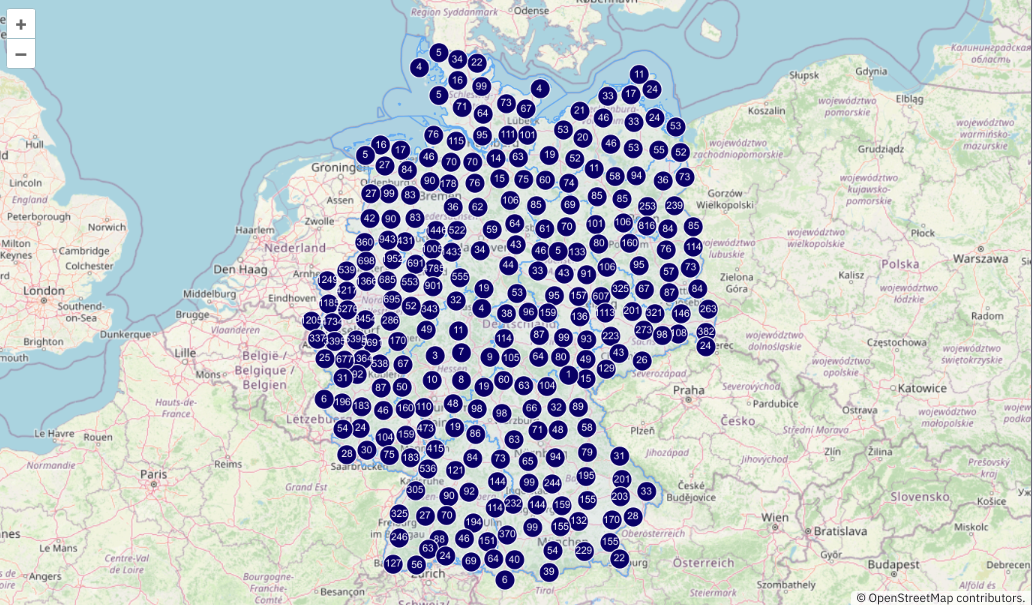
\includegraphics[keepaspectratio]{images/grundwassermessstellen.png}}

Link:
\href{https://correctiv.org/aktuelles/kampf-um-wasser/2022/10/25/klimawandel-grundwasser-in-deutschland-sinkt/}{Grundwasser-Analyse}

\subsection{Projekt-Ideen zum Kennenlernen von
mvp.umwelt.info}\label{projekt-ideen-zum-kennenlernen-von-mvp.umwelt.info}

\begin{itemize}
\tightlist
\item
  Ein weiteres Bundesland auswählen und Grundwasserdaten auf umwelt.info
  finden
\item
  Metadatenanalyse der Grundwasser-Messstellen fortführen
\item
  Wie entwickelt sich der Wasserstand bei Flüssen, Seen, Teichen?
\end{itemize}

Link:
\href{https://correctiv.org/aktuelles/kampf-um-wasser/2022/10/25/klimawandel-grundwasser-in-deutschland-sinkt/}{Grundwasser-Analyse}

\subsection{Bonus-Content}\label{bonus-content}

Auf den folgenden Folien finden sich einige vertiefende Infos zur
Präsentation.

\subsection{💡 Web-UI vs.~API-Zugriff
Zusammenfassung}\label{web-ui-vs.-api-zugriff-zusammenfassung}

\begin{itemize}
\tightlist
\item
  Suche: Zum Erkunden und Verstehen der Daten
\item
  Schnittstelle (API): Für systematische Datenabfragen
\end{itemize}

\subsection{CKAN-API: Bereitstellung von
Metadaten}\label{ckan-api-bereitstellung-von-metadaten}

CKAN (Comprehensive Knowledge Archive Network) ist eine Open
Source-Software zur Katalogisierung und Bereitstellung von Open Data.
\begin{center}

\includegraphics[width=0.7\linewidth,height=0.7\textheight]{images/ckan_logo.pdf}
\end{center}

\subsection{Grundwasser-Atlas:
Beispiel-Visualisierung}\label{grundwasser-atlas-beispiel-visualisierung}

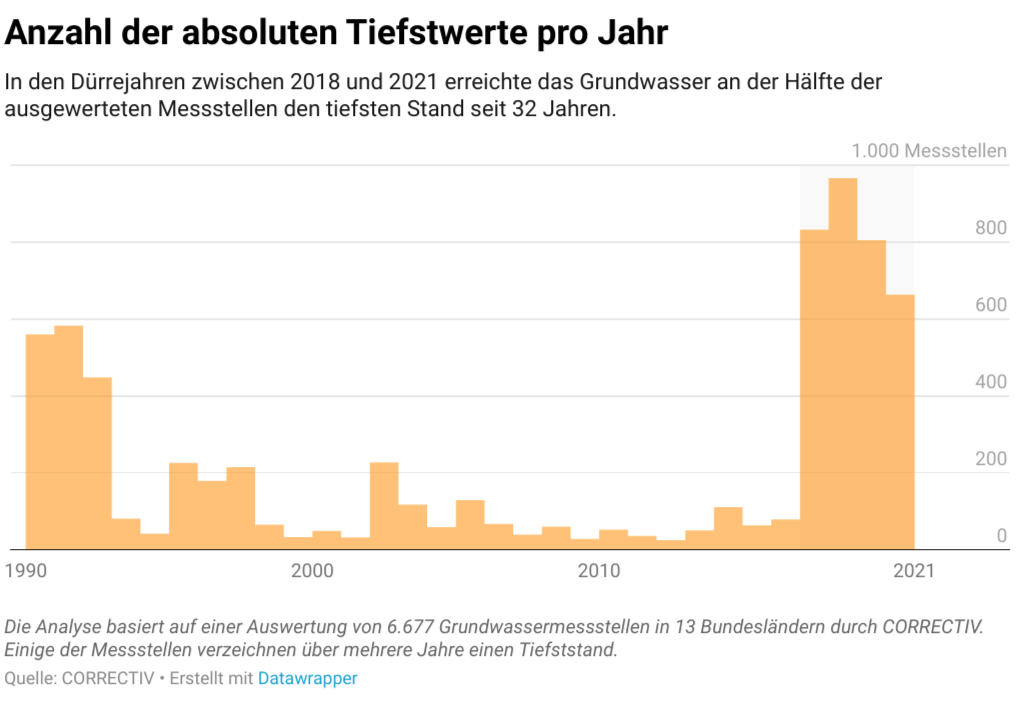
\includegraphics[width=0.8\linewidth,height=0.8\textheight]{images/correctiv_anzahl_tiefstwerte.png}

Quelle:
\href{https://correctiv.org/aktuelles/kampf-um-wasser/2022/10/25/klimawandel-grundwasser-in-deutschland-sinkt/}{CORRECTIV}

Grundwasser-Atlas: Beispielhafte Visualisierung mit Python

\subsection{Grundwassertrends in Deutschland 1990-2021 (Python-Code
verfügbar in
.qmd)}\label{grundwassertrends-in-deutschland-1990-2021-python-code-verfuxfcgbar-in-.qmd}

\begin{Shaded}
\begin{Highlighting}[]
\ImportTok{import}\NormalTok{ plotly.graph\_objects }\ImportTok{as}\NormalTok{ go}

\CommentTok{\# Data}
\NormalTok{trend\_data }\OperatorTok{=}\NormalTok{ [}
\NormalTok{    \{}\StringTok{"name"}\NormalTok{: }\StringTok{"Stark sinkend"}\NormalTok{, }\StringTok{"value"}\NormalTok{: }\DecValTok{533}\NormalTok{, }\StringTok{"color"}\NormalTok{: }\StringTok{"\#E9650E"}\NormalTok{, }\StringTok{"percent"}\NormalTok{: }\FloatTok{8.0}\NormalTok{\},}
\NormalTok{    \{}\StringTok{"name"}\NormalTok{: }\StringTok{"Leicht sinkend"}\NormalTok{, }\StringTok{"value"}\NormalTok{: }\DecValTok{1087}\NormalTok{, }\StringTok{"color"}\NormalTok{: }\StringTok{"\#FFB727"}\NormalTok{, }\StringTok{"percent"}\NormalTok{: }\FloatTok{16.3}\NormalTok{\},}
\NormalTok{    \{}\StringTok{"name"}\NormalTok{: }\StringTok{"Kein starker Trend"}\NormalTok{, }\StringTok{"value"}\NormalTok{: }\DecValTok{4035}\NormalTok{, }\StringTok{"color"}\NormalTok{: }\StringTok{"\#eeeeee"}\NormalTok{, }\StringTok{"percent"}\NormalTok{: }\FloatTok{60.4}\NormalTok{\},}
\NormalTok{    \{}\StringTok{"name"}\NormalTok{: }\StringTok{"Leicht steigend"}\NormalTok{, }\StringTok{"value"}\NormalTok{: }\DecValTok{529}\NormalTok{, }\StringTok{"color"}\NormalTok{: }\StringTok{"\#71B5FE"}\NormalTok{, }\StringTok{"percent"}\NormalTok{: }\FloatTok{7.9}\NormalTok{\},}
\NormalTok{    \{}\StringTok{"name"}\NormalTok{: }\StringTok{"Stark steigend"}\NormalTok{, }\StringTok{"value"}\NormalTok{: }\DecValTok{493}\NormalTok{, }\StringTok{"color"}\NormalTok{: }\StringTok{"\#0163CB"}\NormalTok{, }\StringTok{"percent"}\NormalTok{: }\FloatTok{7.4}\NormalTok{\}}
\NormalTok{]}

\CommentTok{\# Create figure}
\NormalTok{fig }\OperatorTok{=}\NormalTok{ go.Figure()}

\CommentTok{\# Add bar chart}
\NormalTok{fig.add\_trace(}
\NormalTok{    go.Bar(}
\NormalTok{        x}\OperatorTok{=}\NormalTok{[d[}\StringTok{"name"}\NormalTok{] }\ControlFlowTok{for}\NormalTok{ d }\KeywordTok{in}\NormalTok{ trend\_data],}
\NormalTok{        y}\OperatorTok{=}\NormalTok{[d[}\StringTok{"value"}\NormalTok{] }\ControlFlowTok{for}\NormalTok{ d }\KeywordTok{in}\NormalTok{ trend\_data],}
\NormalTok{        marker\_color}\OperatorTok{=}\NormalTok{[d[}\StringTok{"color"}\NormalTok{] }\ControlFlowTok{for}\NormalTok{ d }\KeywordTok{in}\NormalTok{ trend\_data],}
\NormalTok{        text}\OperatorTok{=}\NormalTok{[d[}\StringTok{"value"}\NormalTok{] }\ControlFlowTok{for}\NormalTok{ d }\KeywordTok{in}\NormalTok{ trend\_data],}
\NormalTok{        textposition}\OperatorTok{=}\StringTok{\textquotesingle{}auto\textquotesingle{}}\NormalTok{,}
\NormalTok{    )}
\NormalTok{)}

\CommentTok{\# Update layout}
\NormalTok{fig.update\_layout(}
\NormalTok{    title\_text}\OperatorTok{=}\StringTok{"Grundwassertrends in Deutschland 1990{-}2021"}\NormalTok{,}
\NormalTok{    showlegend}\OperatorTok{=}\VariableTok{False}\NormalTok{,}
\NormalTok{    height}\OperatorTok{=}\DecValTok{500}\NormalTok{,  }\CommentTok{\# Reduced height since we only have one chart now}
\NormalTok{    paper\_bgcolor}\OperatorTok{=}\StringTok{\textquotesingle{}black\textquotesingle{}}\NormalTok{,}
\NormalTok{    plot\_bgcolor}\OperatorTok{=}\StringTok{\textquotesingle{}black\textquotesingle{}}\NormalTok{,}
\NormalTok{    font}\OperatorTok{=}\BuiltInTok{dict}\NormalTok{(color}\OperatorTok{=}\StringTok{\textquotesingle{}white\textquotesingle{}}\NormalTok{),}
\NormalTok{    template}\OperatorTok{=}\StringTok{\textquotesingle{}plotly\_dark\textquotesingle{}}
    \CommentTok{\# annotations=[}
    \CommentTok{\#     dict(}
    \CommentTok{\#         text=f"Gesamtzahl der Messstellen: \{sum(d[\textquotesingle{}value\textquotesingle{}] for d in trend\_data)\}",}
    \CommentTok{\#         xref="paper",}
    \CommentTok{\#         yref="paper",}
    \CommentTok{\#         x=0.5,}
    \CommentTok{\#         y=1.1,}
    \CommentTok{\#         showarrow=False,}
    \CommentTok{\#         font=dict(size=16, color=\textquotesingle{}white\textquotesingle{})}
    \CommentTok{\#     )}
    \CommentTok{\# ]}
\NormalTok{)}

\CommentTok{\# Update axes}
\NormalTok{fig.update\_xaxes(showgrid}\OperatorTok{=}\VariableTok{True}\NormalTok{, gridwidth}\OperatorTok{=}\DecValTok{1}\NormalTok{, gridcolor}\OperatorTok{=}\StringTok{\textquotesingle{}rgba(128,128,128,0.2)\textquotesingle{}}\NormalTok{)}
\NormalTok{fig.update\_yaxes(showgrid}\OperatorTok{=}\VariableTok{True}\NormalTok{, gridwidth}\OperatorTok{=}\DecValTok{1}\NormalTok{, gridcolor}\OperatorTok{=}\StringTok{\textquotesingle{}rgba(128,128,128,0.2)\textquotesingle{}}\NormalTok{)}

\CommentTok{\# Make it responsive}
\NormalTok{config }\OperatorTok{=}\NormalTok{ \{}
    \StringTok{\textquotesingle{}responsive\textquotesingle{}}\NormalTok{: }\VariableTok{True}\NormalTok{,}
    \StringTok{\textquotesingle{}displayModeBar\textquotesingle{}}\NormalTok{: }\VariableTok{False}
\NormalTok{\}}

\NormalTok{fig.show(config}\OperatorTok{=}\NormalTok{config)}
\end{Highlighting}
\end{Shaded}

\begin{verbatim}
Unable to display output for mime type(s): text/html
\end{verbatim}

\begin{verbatim}
Unable to display output for mime type(s): text/html
\end{verbatim}




\end{document}
